\hypertarget{P1}{}
\begin{solution}{normal} % 1
For an overcurrent protection, there are two fuses connected in parallel: fuse $A$ has resistance $R_A= 1\;\Omega$ and maximal current (by which it melts) $I_{A_\text{max}}= 1 \;\text{A}$; fuse $B$ has resistance $R_B= 2\;\Omega$ and maximal current (by which it melts) $I_{B_\text{max}}= 1.2\;\text{A}$. What is the maximal total current for such a system of fuses? What is the total current when the fuse $B$ is substituted with a fuse $C$ which has $R_C= 2\;\Omega$ and $I_{C_\text{max}}= 1.7\;\text{A}$? (Kalda Circuits P32)
\end{solution}

\hypertarget{P2}{}
\begin{solution}{normal} % 2
The measuring range of a microammeter is $100\;\mu\text{A}$. At this current, there is a voltage drop of $0.1\;\text{V}$ across the terminals of the ammeter. How should a resistor be connected and how large should its resistance be to mimic a) a voltmeter with a measuring range of $100\;\text{V}$ and b) an ammeter with a measuring range of $10\;\text{A}$?
\end{solution}

\hypertarget{P3}{}
\begin{solution}{normal} % 3
A light bulb with power $100\;\text{W}$ is designed for an input voltage of $110\;\text{V}$. What is the resistance of the resistor that should be connected in series to the light bulb such that it has the same brightness with an input voltage of $127\;\text{V}$?
\end{solution}

\hypertarget{P4}{}
\begin{solution}{normal} % 4
Eight identical fluorescent lamps are connected to a constant voltage source as shown in the figure below. There is a resistor in series with the voltage source with resistance equal to that of a single lamp. Does the power emitted by the lamps increase or decrease if one of the lamps burn out? If multiple lamps burn out? Ignore the temperature dependence of the resistance of the lamps. (Similar to Kalda Circuits P41)
\begin{center}
    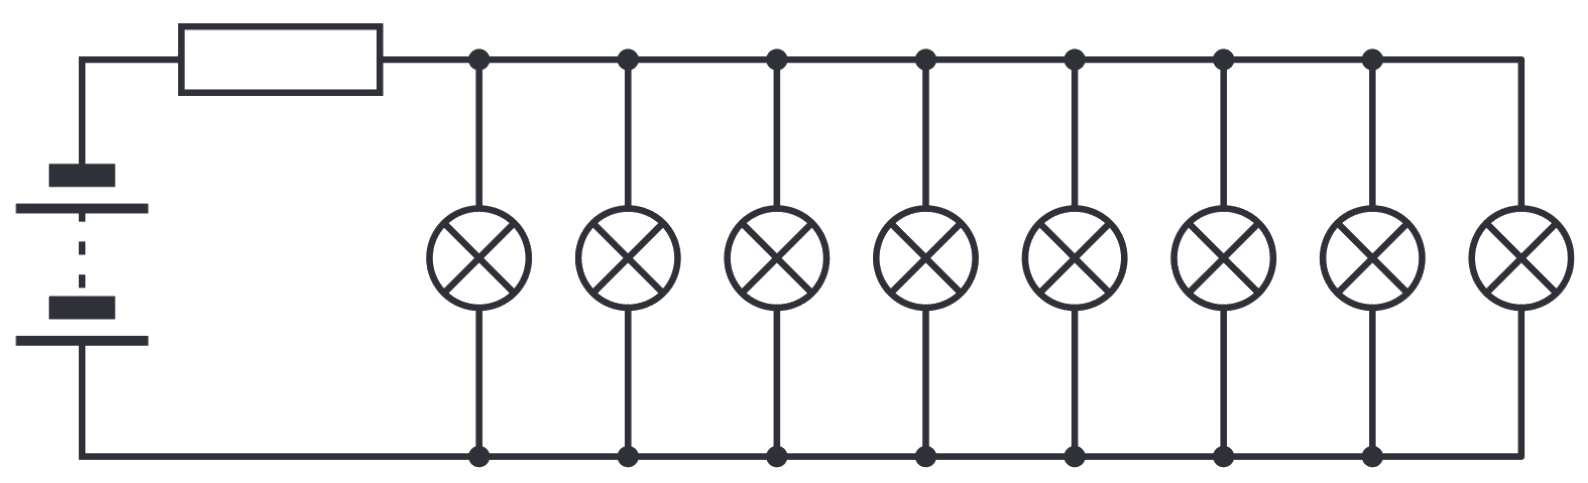
\includegraphics[width=0.55\textwidth]{S1 Figures/S1-4.png}
\end{center}
\end{solution}

\hypertarget{P5}{}
\begin{solution}{normal} % 5
A piece of wire with total resistance $R_0$ is shaped into a closed ring, as shown in the figure below. Two contacts are soldered onto the side of this ring. Determine the resistance between the two contacts if $\alpha=120\degree$.
\begin{center}
    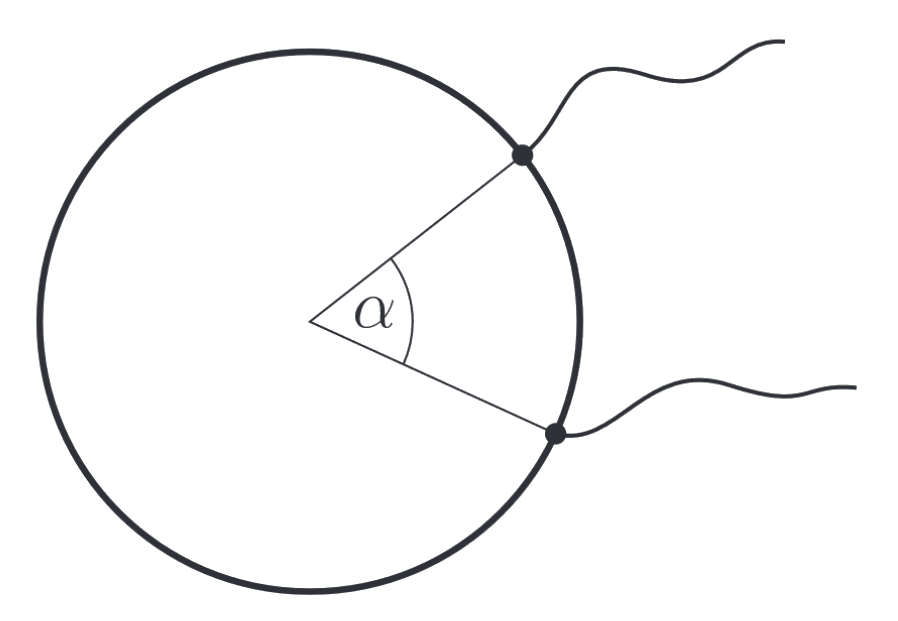
\includegraphics[width=0.31\textwidth]{S1 Figures/S1-5.png}
\end{center}
\end{solution}

\hypertarget{P6}{}
\begin{solution}{normal} % 6 ? kinda unsure about translation
To determine the resistivity of ocean water, a marine scientist immerses a cable of length $50\;\text{mm}$ in the water. The cable consists of two concentric cylindrical electrodes with inner diameter $40\;\text{mm}$ and outer diameter $45\;\text{mm}$. If the resistance between the electrodes is $9\;\Omega$, determine the resistivity of the water.
\end{solution}

\hypertarget{P7}{}
\begin{solution}{normal} % 7
A uniform wire of cross-sectional area $A_0=1\;\text{mm}^2$ had a millimetre scale marked on it: an array of streaks with inter-streak distance $a_0=1\;\text{mm}$ covered the entire length of the wire. The wire was stretched in a non-uniform way, so that the inter-streak distance $a$ is now a function of the distance $l$ from one end of the wire (as measured after the stretching), see figure.The new length of the wire is $L=4\;\text{m}$. Using the graph, determine the electrical resistance $R$ of the stretched wire assuming that the resistivity of the wire material is $\rho=1.0\times10^{-6}\;\Omega\;\text{m}$. During the stretching, the density of the wire material remains constant. \textit{Note:} If a problem contains graphical data, the solution usually comes down to area of the graph, its slope, or intersections in the graph. (Kalda Circuits P1)
\begin{center}
    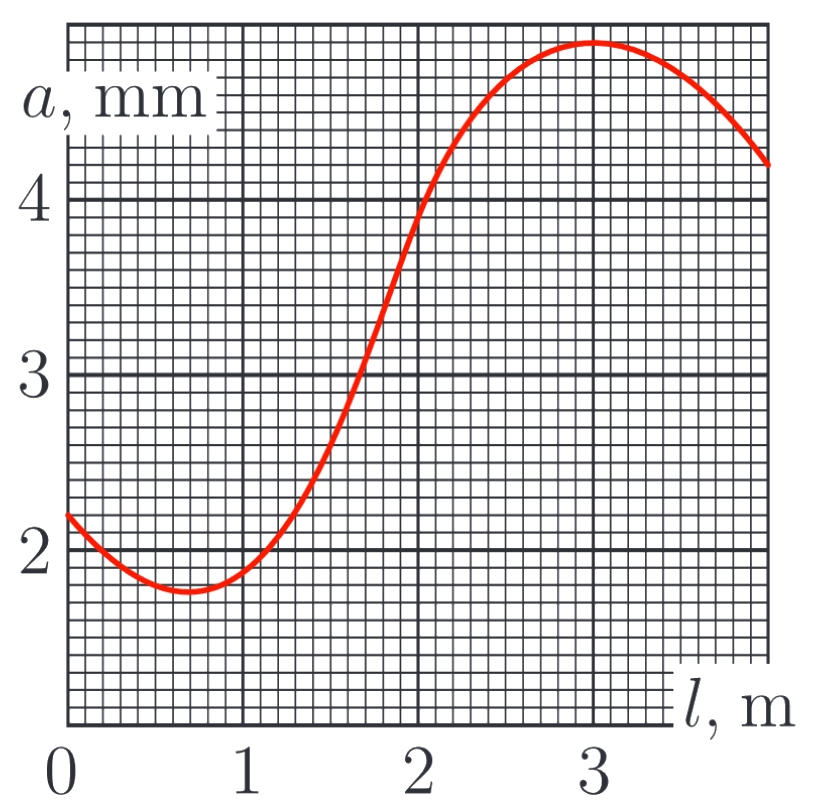
\includegraphics[width=0.48\textwidth]{S1 Figures/S1-7.png}
\end{center}
\end{solution}

\hypertarget{P8}{}
\begin{solution}{normal} % 8
The figure below shows part of a larger circuit. Four identical ammeters, each with an internal resistance of $100\;\Omega$, are connected to the circuit. The readings on the first and second ammeters are $3\;\text{mA}$ and $\text{5mA}$, respectively. Determine the resistance of resistor $R$.
\begin{center}
    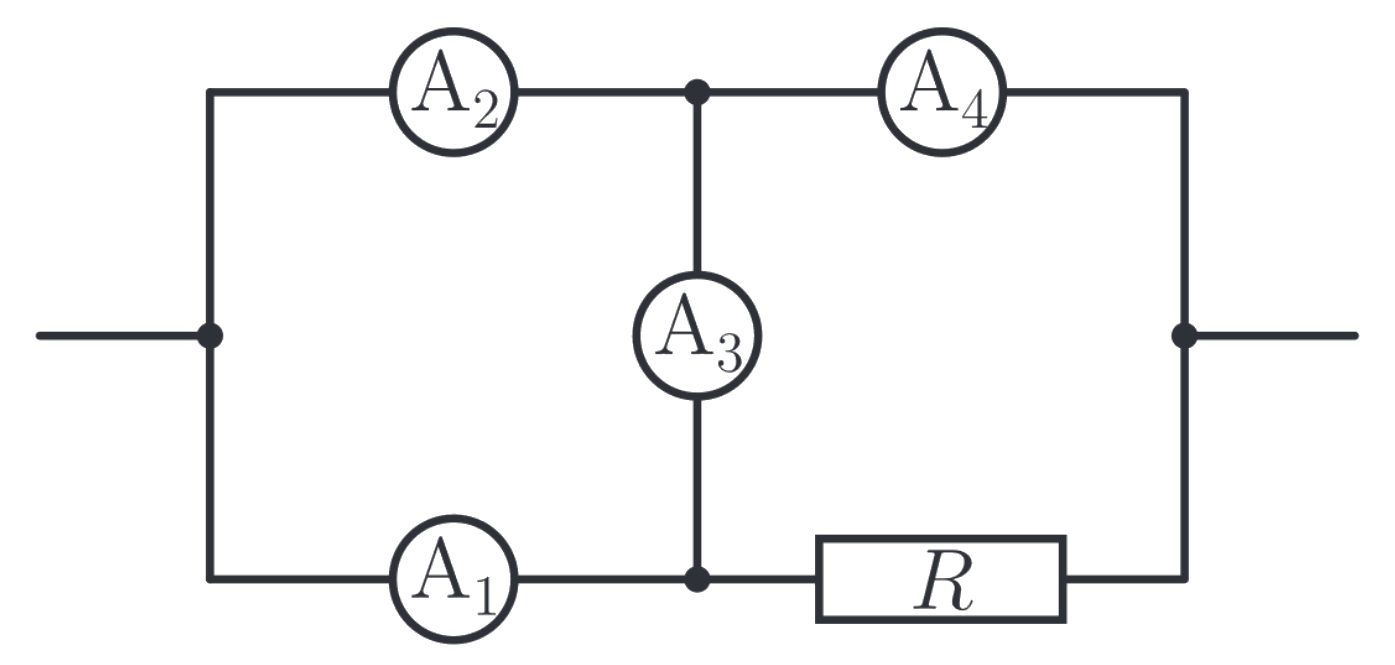
\includegraphics[width=0.55\textwidth]{S1 Figures/S1-8.png}
\end{center}
\end{solution}

\hypertarget{P9}{}
\begin{solution}{normal} % 9
The circuit in the figure below consists of three identical voltmeters and three identical resistors. If the reading on the first voltmeter is $19\;\text{V}$ and the reading on the third voltmeter is $9\;\text{V}$, find the reading on the second voltmeter. (Similar to Kalda Circuits P39)
\begin{center}
    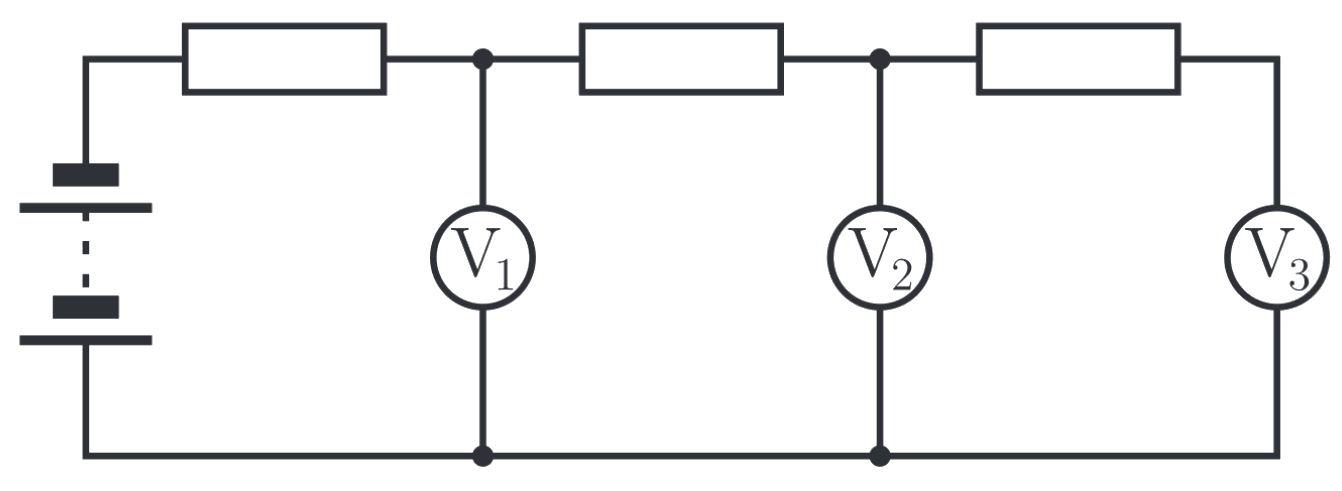
\includegraphics[width=0.65\textwidth]{S1 Figures/S1-9.png}
\end{center}
\end{solution}

\hypertarget{P10}{}
\begin{solution}{normal} % 10
Determine the resistance of the circuit shown below using both the potential and current methods. \textit{Note:} To simplify the statements, you may consider a current of $1\;\text{A}$ passing through the circuit or that the output terminals are connected to a $1\;\text{V}$ voltage source. In the first case, the voltage drop between the ends of the circuit is numerically equal to the effective resistance, and in the second case, the current through the circuit is numerically equal to the inverse of the resistance. (Similar to Kalda Circuits P1)
\begin{center}
    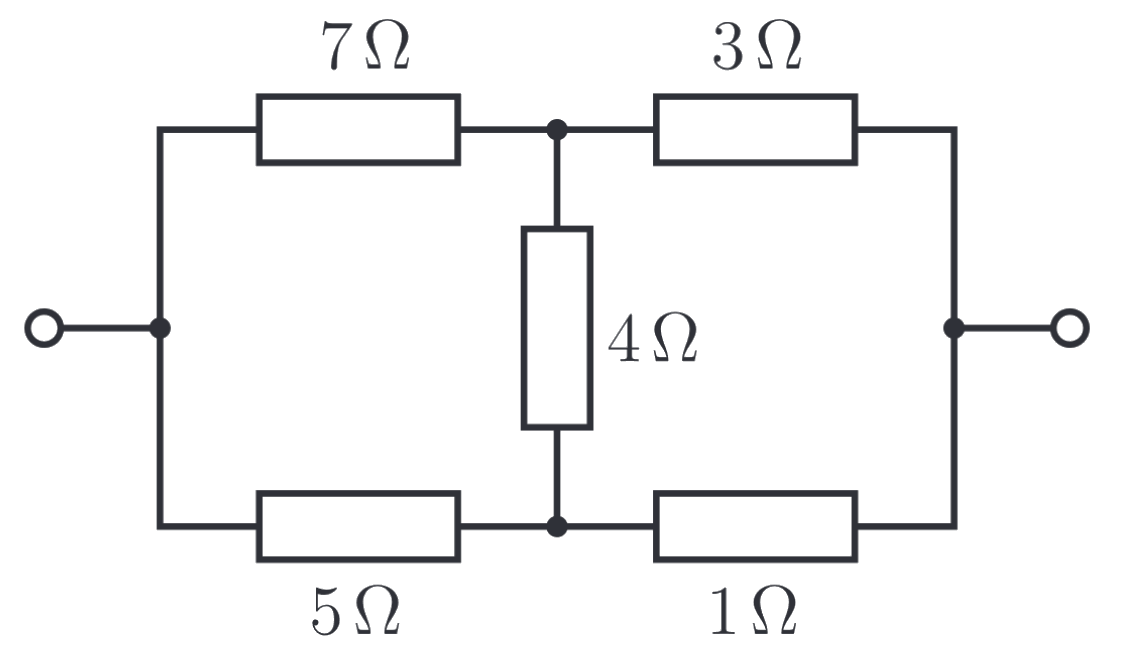
\includegraphics[width=0.55\textwidth]{S1 Figures/S1-10.png}
\end{center}
\end{solution}

\hypertarget{P11}{}
\begin{solution}{normal} % 11
In the figure, $R_1/R_2=4$. If we add a lamp as shown in the figure below, the current through $R_1$ will increase by $\Delta I= 0.1\;\text{A}$. Determine the current through the lamp. (Kalda Circuits P2)
\begin{center}
    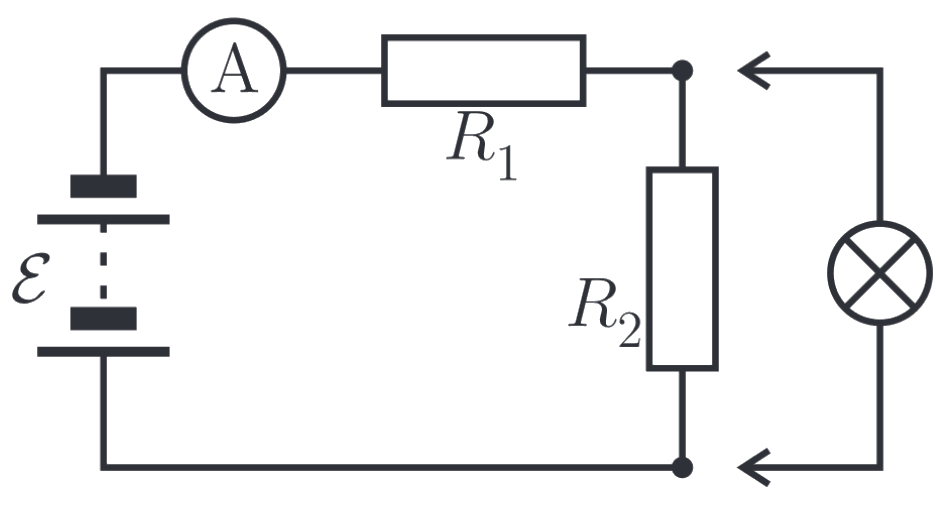
\includegraphics[width=0.5\textwidth]{S1 Figures/S1-11.png}
\end{center}
\end{solution}

\hypertarget{P12}{}
\begin{solution}{normal} % 12
Determine the current through resistor $R_3$ in the circuit shown below.
\begin{center}
    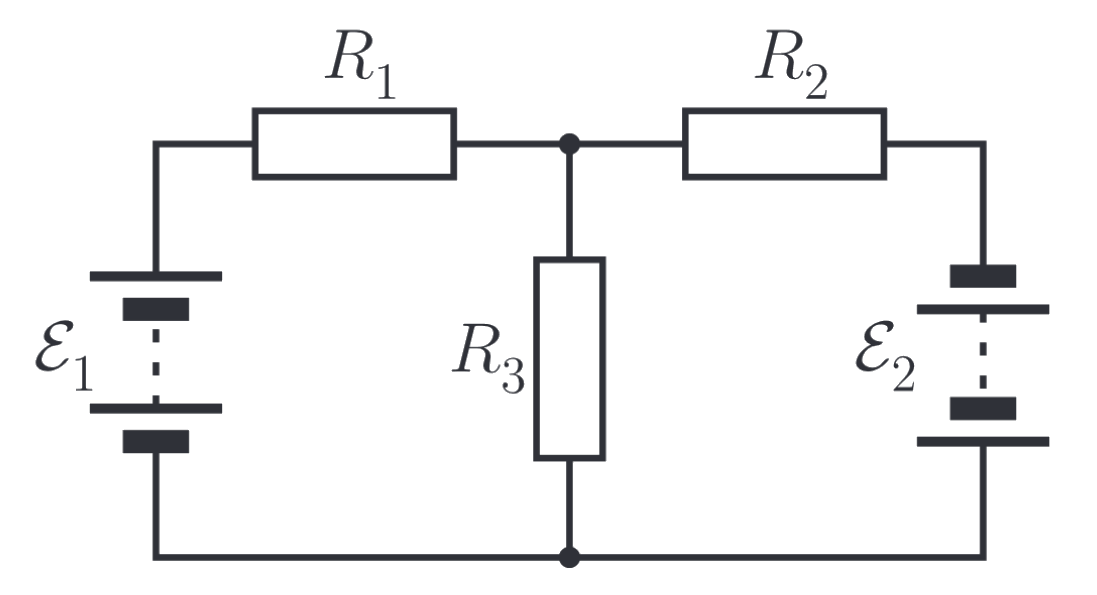
\includegraphics[width=0.6\textwidth]{S1 Figures/S1-12.png}
\end{center}
\end{solution}

\hypertarget{P13}{}
\begin{solution}{normal} % 13
Determine the current through the $8\;\Omega$ resistor. (Similar to Kalda Circuits P12)
\begin{center}
    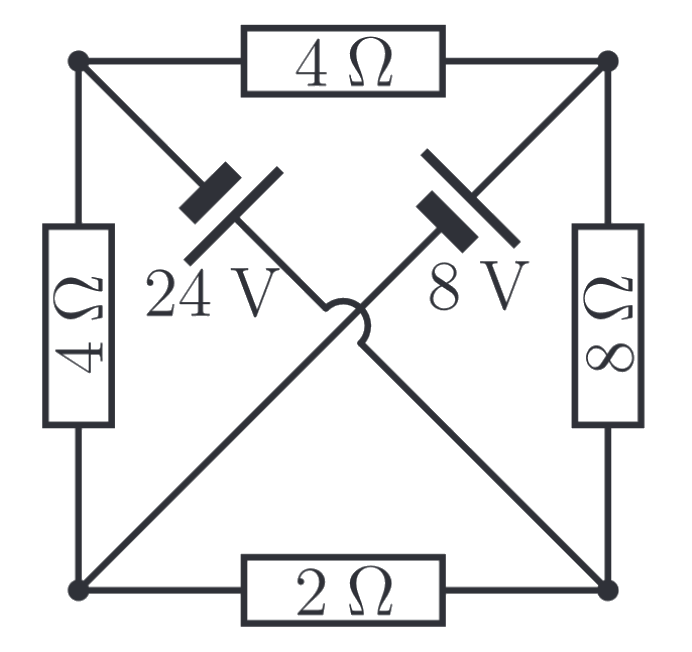
\includegraphics[width=0.38\textwidth]{S1 Figures/S1-13.png}
\end{center}
\end{solution}

\hypertarget{P14}{}
\begin{solution}{normal} % 14
Determine the currents through the batteries. (Kalda Circuits P9)
\begin{center}
    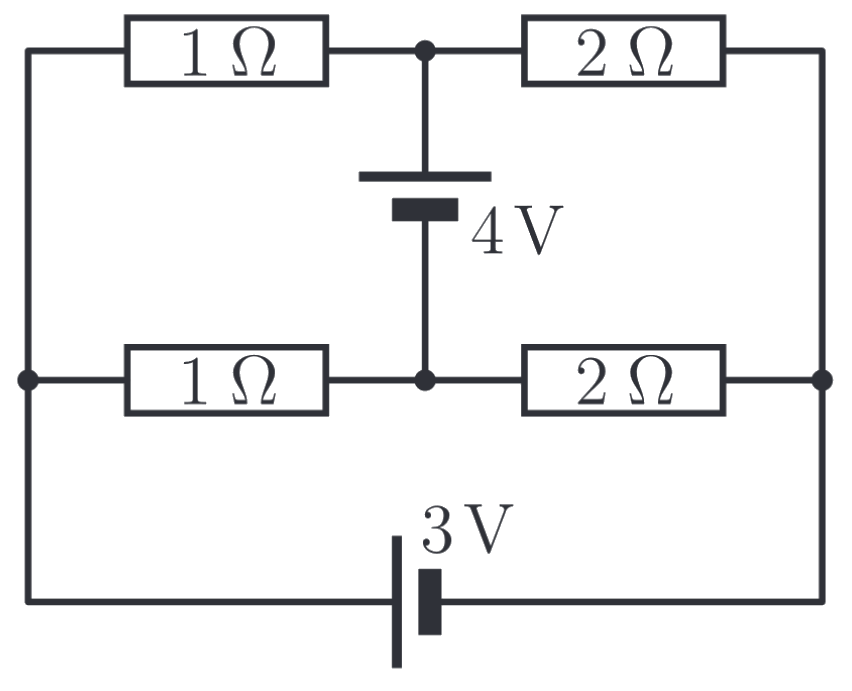
\includegraphics[width=0.45\textwidth]{S1 Figures/S1-14.png}
\end{center}
\end{solution}

\hypertarget{P15}{}
\begin{solution}{normal} % 15
Determine the resistance of the circuit shown below.
\begin{center}
    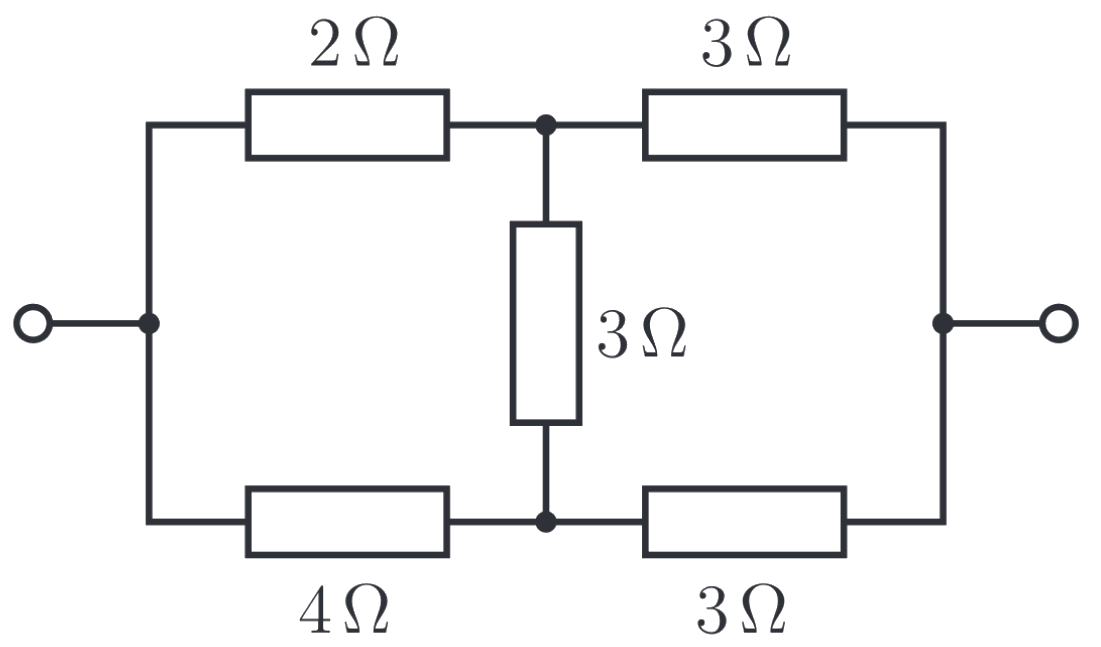
\includegraphics[width=0.6\textwidth]{S1 Figures/S1-15.png}
\end{center}
\end{solution}

\hypertarget{P16}{}
\begin{solution}{normal} % 16 ? kinda unsure about translation
To make Christmas decorations, Juku took 10 identical light bulbs (with a rated voltage of $3\;\text{V}$ and a rated power of $0.6\;\text{W}$), and a rectifier with terminal voltage of $5\;\text{V}$. Based on this, he designed the circuit shown below. He then calculated the necessary value of $R$ such that the voltage across the bulbs is the same as their rated voltage. However, when the rectifier was switched on, the bulbs were still dimmer than expected. Further testing showed that the terminal voltage of the rectifier had dropped to $4\;\text{V}$ and that the voltage across the bulbs had dropped to $2.4\;\text{V}$. How large should $R$ be to light the bulbs to their normal brightness?
\begin{center}
    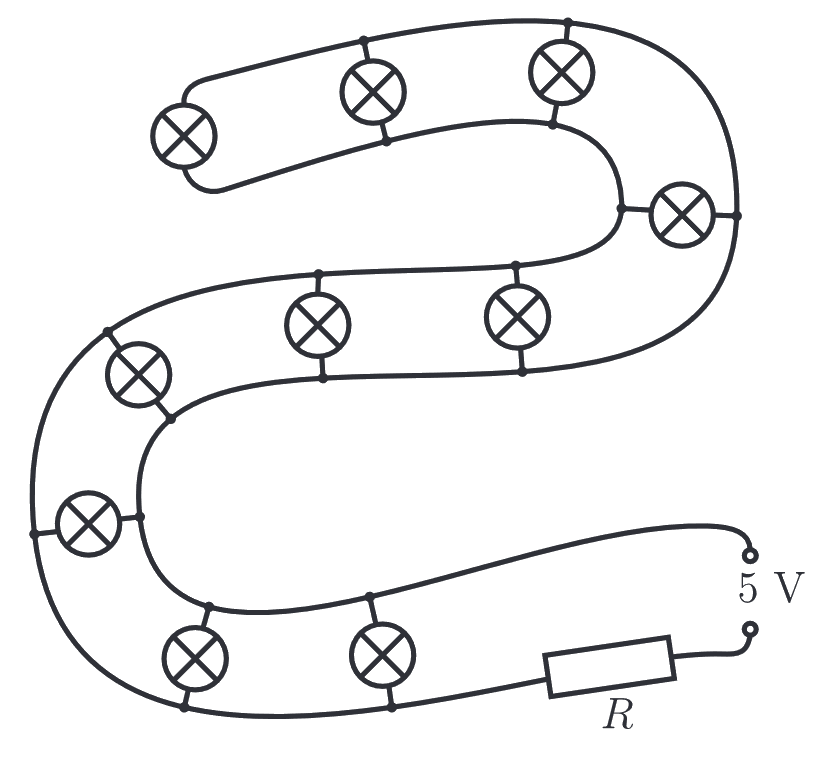
\includegraphics[width=0.7\textwidth]{S1 Figures/S1-16.png}
\end{center}
\end{solution}

\hypertarget{P17}{}
\begin{solution}{normal} % 17
The maximum current ($\mathcal{E}/r$) is obtained from the voltage source if the resistance of the external circuit is zero (i.e. the terminals are short-circuited). However, in this case, the electrical power consumed in the external circuit is also zero. Show that the maximum net power is obtained from a voltage source if the external circuit resistance is equal to the internal resistance of the source.
\end{solution}

\hypertarget{P18}{}
\begin{solution}{normal} % 18
What is the maximum power that can be drawn from the output terminals of the circuits shown below Problem 19?
\end{solution}

\hypertarget{P19}{}
\begin{solution}{normal} % 19
Solve the previous problem using equivalent circuits.
\begin{center}
    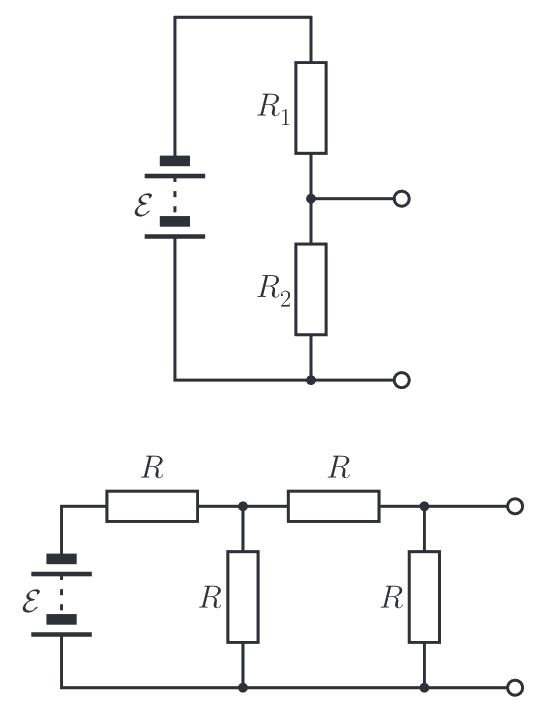
\includegraphics[width=0.42\textwidth]{S1 Figures/S1-18-19.png}
\end{center}
\end{solution}

\hypertarget{P20}{}
\begin{solution}{normal} % 20
In the circuit shown below, determine the voltage at the output terminals and the current through a $10\;\text{k}\Omega$ resistor if the switch $K$ is a) open; b) closed.
\begin{center}
    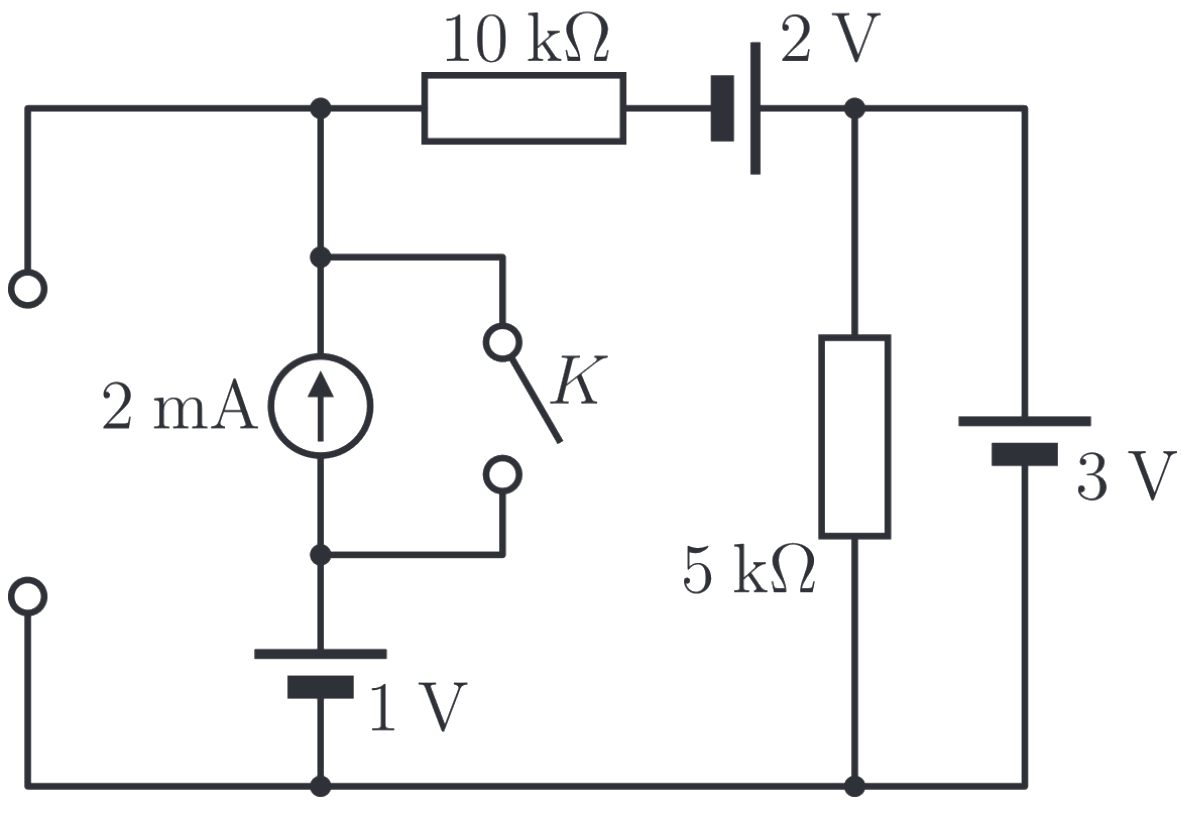
\includegraphics[width=0.45\textwidth]{S1 Figures/S1-20.png}
\end{center}
\end{solution}

\hypertarget{P21}{}
\begin{solution}{normal} % 21
$N$ batteries are connected in parallel. The $i^\text{th}$ source has emf $\mathcal{E}_i$ and internal resistance $r_i$. What are the effective emf and internal resistance of the combined voltage source?
\end{solution}

\hypertarget{P22}{}
\begin{solution}{normal} % 22
Using the theorem below, resolve Problem 12.
\blfootnote{Millman's theorem states that if we have multiple branches in parallel with one voltage source of emf $\mathcal{E}_i$ and one resistor of resistance $R_i$ on each branch, the total emf is given by $U=\left(\sum_i\frac{\mathcal{E}_i}{R_i}\right)/\left(\sum_i\frac{1}{R_i}\right)$}
\end{solution}

\hypertarget{P23}{}
\begin{solution}{normal} % 23
Determine the resistance of the following circuits. (Kalda Circuits P4, P18)
\begin{center}
    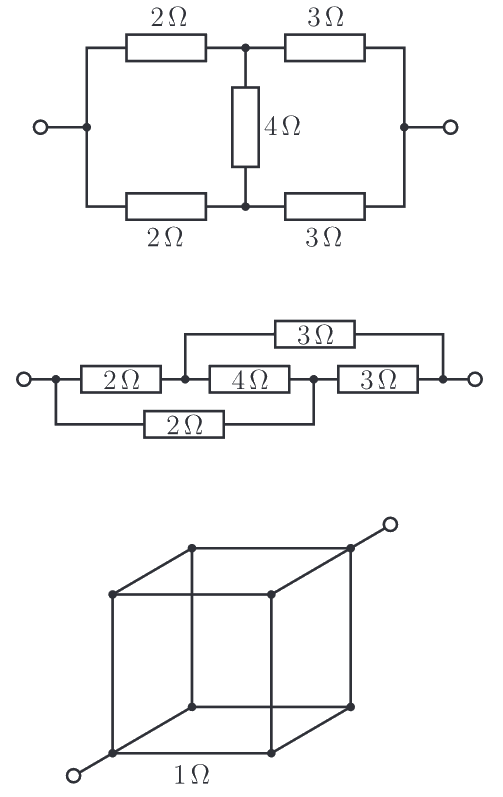
\includegraphics[width=0.6\textwidth]{S1 Figures/S1-23.png}
\end{center}
\end{solution}

\hypertarget{P24}{}
\begin{solution}{normal} % 24
Determine the resistance of the following circuit.
\begin{center}
    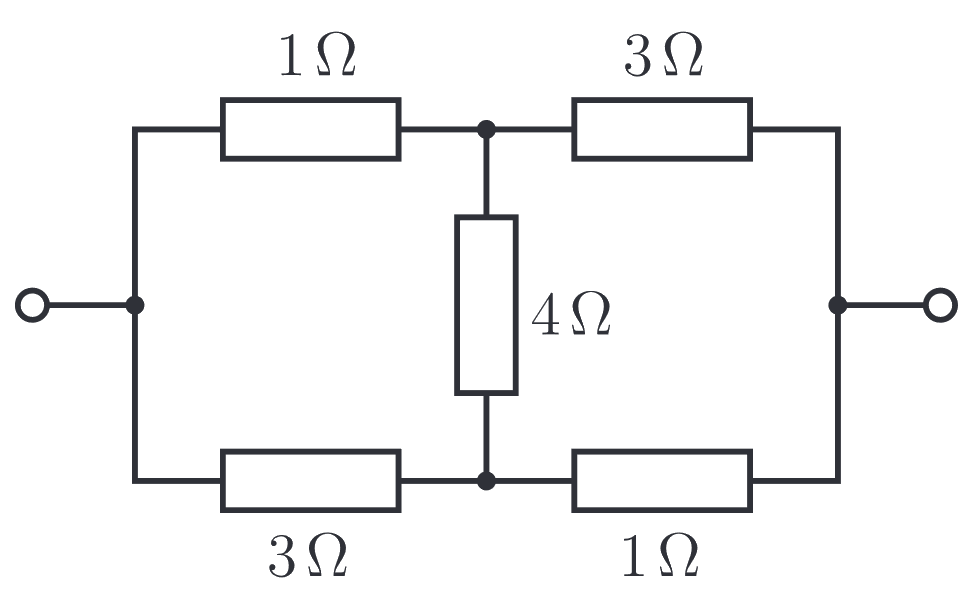
\includegraphics[width=0.55\textwidth]{S1 Figures/S1-24.png}
\end{center}
\end{solution}

\hypertarget{P25}{}
\begin{solution}{normal} % 25
Assuming ideal batteries, determine the currents through all resistors in the following circuit. (Similar to Kalda Circuits P12)
\begin{center}
    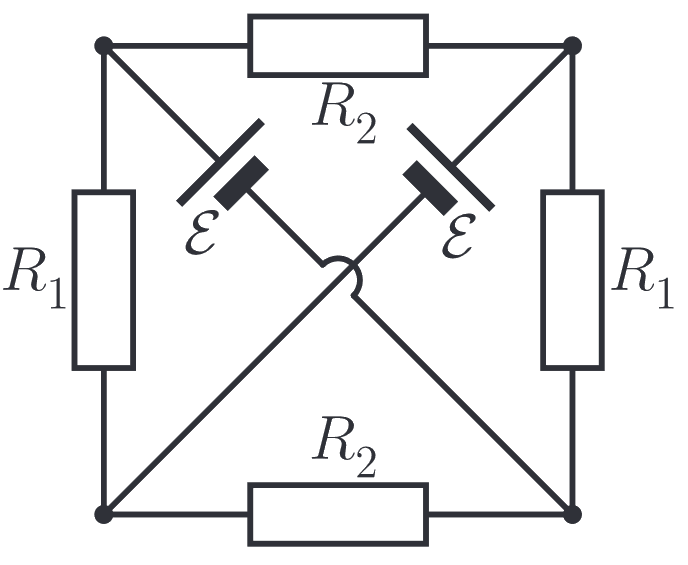
\includegraphics[width=0.4\textwidth]{S1 Figures/S1-25.png}
\end{center}
\end{solution}

\hypertarget{P26}{}
\begin{solution}{normal} % 26
Determine the resistance between any 2 terminals in the circuit shown below.
\begin{center}
    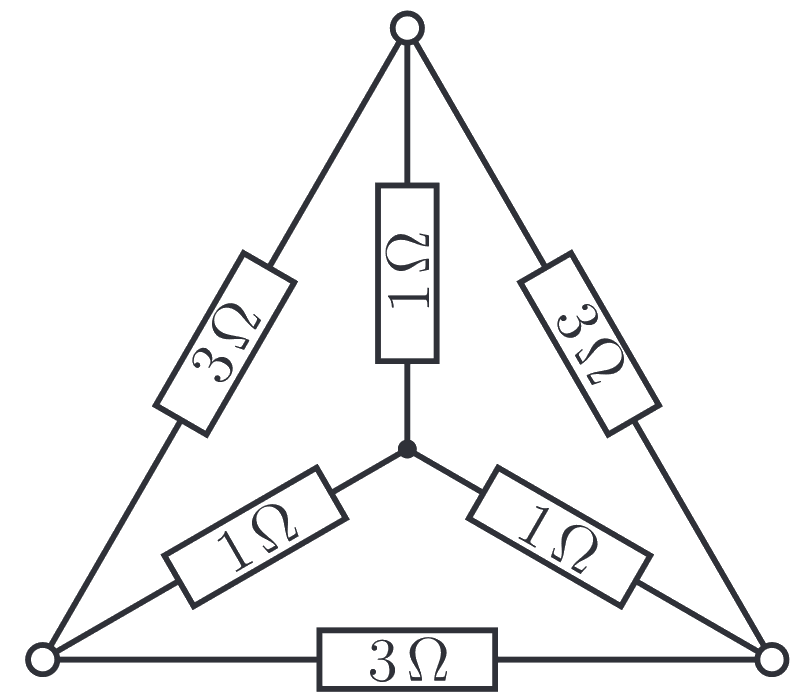
\includegraphics[width=0.45\textwidth]{S1 Figures/S1-26.png}
\end{center}
\end{solution}

\hypertarget{P27}{}
\begin{solution}{normal} % 27
Determine the reading of the ideal ammeter in the circuit below. (Kalda Circuits P36)
\begin{center}
    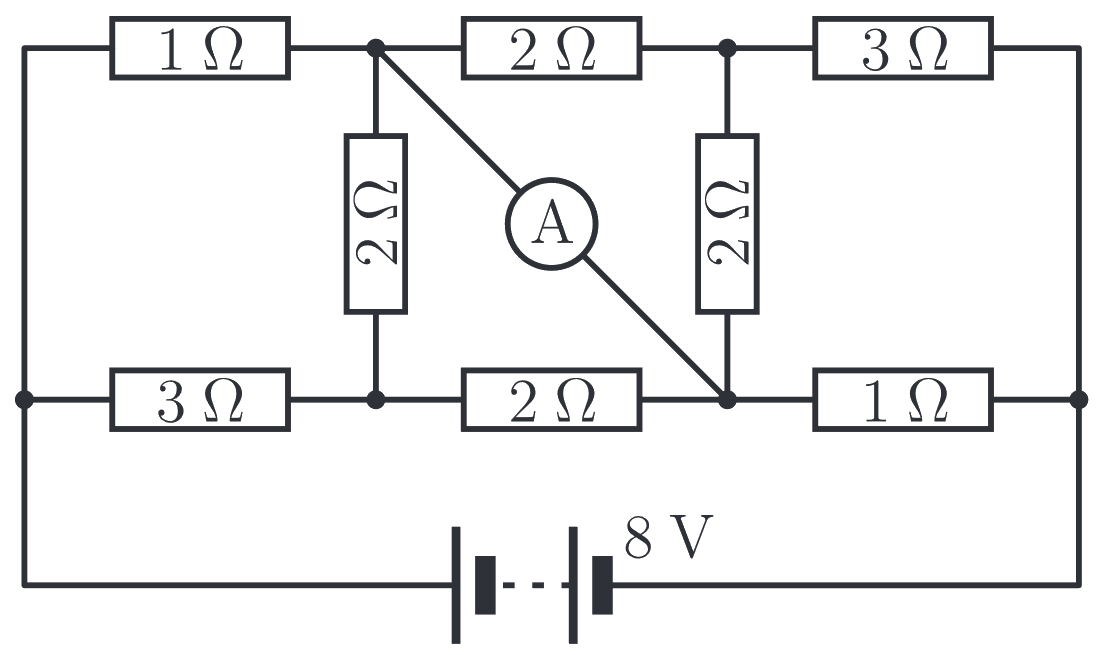
\includegraphics[width=0.6\textwidth]{S1 Figures/S1-27.png}
\end{center}
\end{solution}

\hypertarget{P28}{}
\begin{solution}{normal} % 28
Determine the readings on the ideal ammeter and ideal voltmeter in the following circuit.
\begin{center}
    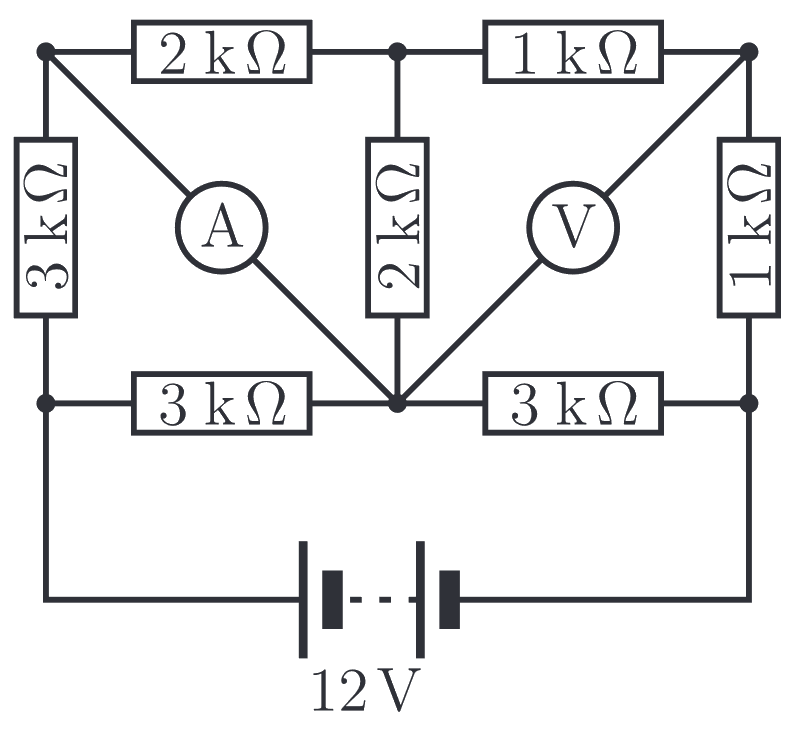
\includegraphics[width=0.45\textwidth]{S1 Figures/S1-28.png}
\end{center}
\end{solution}

\hypertarget{P29}{}
\begin{solution}{normal} % 29
Determine the resistance of the following infinite circuit. (Kalda Circuits P16)
\begin{center}
    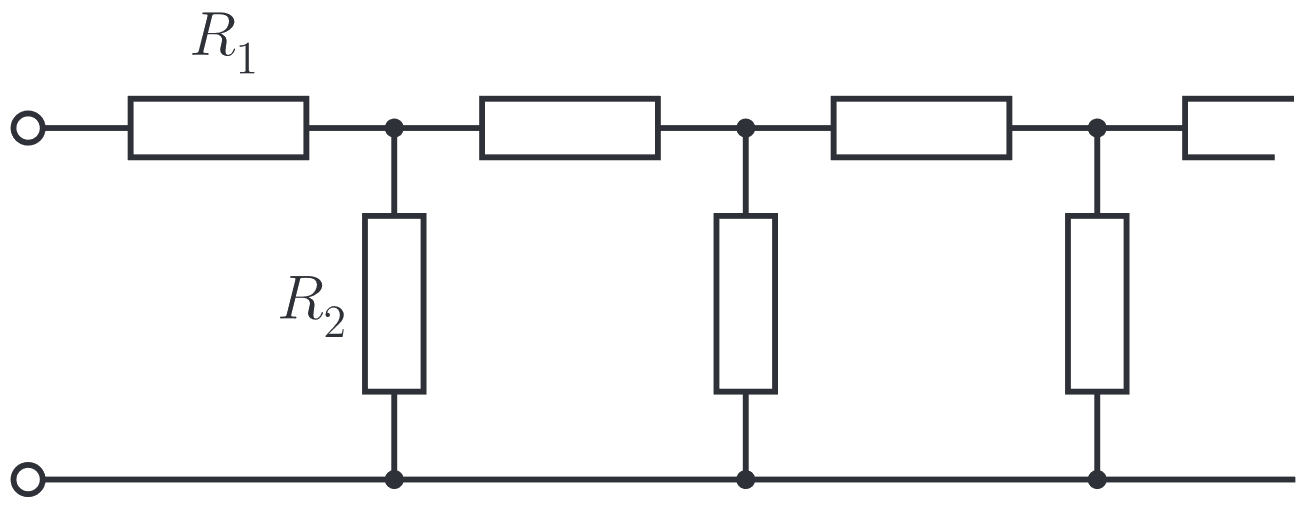
\includegraphics[width=0.7\textwidth]{S1 Figures/S1-29.png}
\end{center}
\end{solution}

\hypertarget{P30}{}
\begin{solution}{normal} % 30
Determine the electromotive force and internal resistance of the following system of batteries. (Kalda Circuits P17)
\begin{center}
    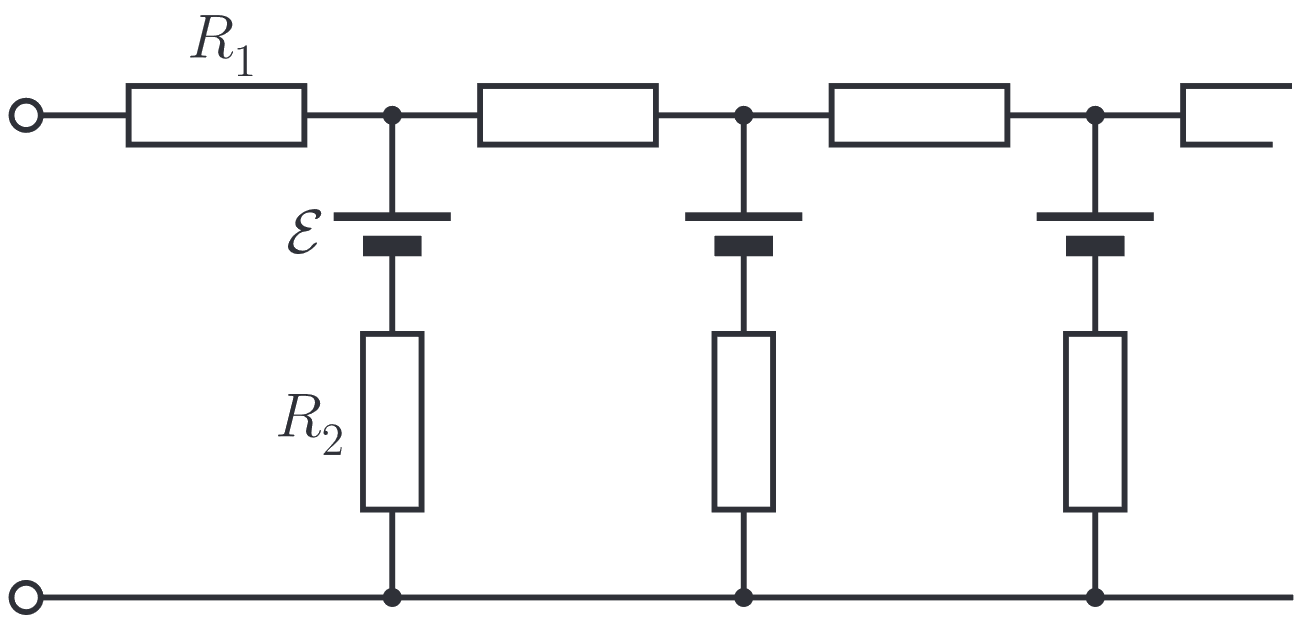
\includegraphics[width=0.7\textwidth]{S1 Figures/S1-30.png}
\end{center}
\end{solution}

\hypertarget{P31}{}
\begin{solution}{normal} % 31 ? Not really sure about the instructions part
Determine the resistance between two neigbouring nodes in an infinite triangular lattice, as shown in the figure below. The resistance of the wire connecting any two neighbouring nodes is $1\;\Omega$. \textit{Instructions:} Let $C$ be a node that is infinitely far from nodes $A$ and $B$. Now consider the currents flowing between these nodes.
\begin{center}
    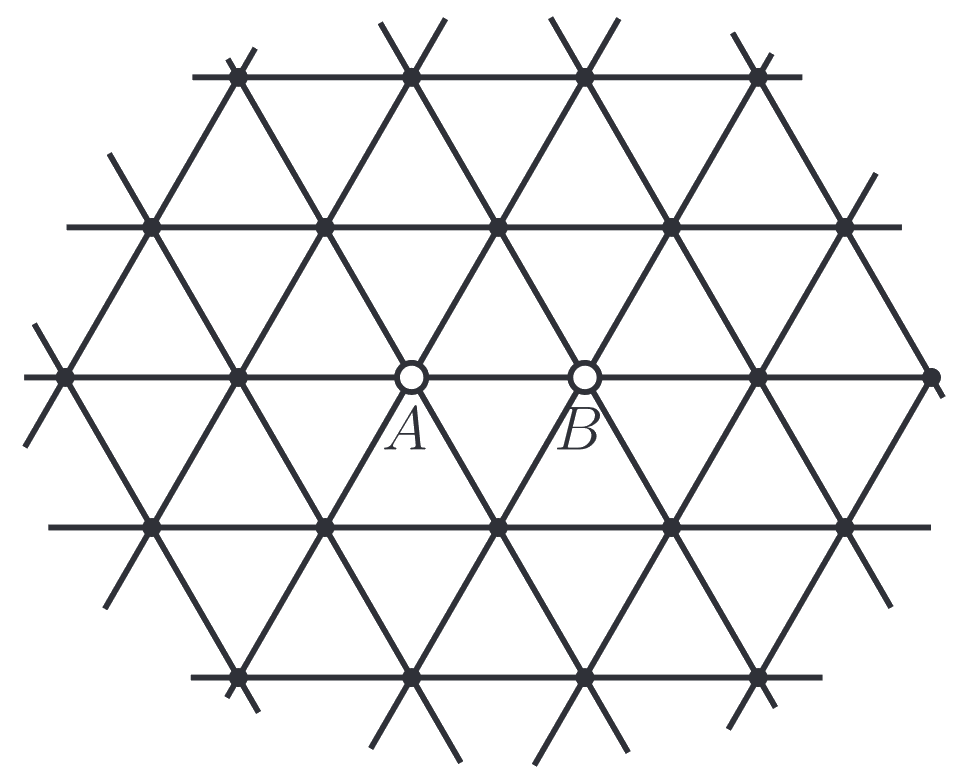
\includegraphics[width=0.5\textwidth]{S1 Figures/S1-31.png}
\end{center}
\end{solution}

\hypertarget{P32}{}
\begin{solution}{normal} % 32
Determine the resistance between two neighbouring nodes $A$ and $B$ of an infinite cubic lattice assuming that the edges of the lattice are made of wire, and the resistance of each edge is $1\;\Omega$. (Kalda Circuits P45)
\end{solution}

\hypertarget{P33}{}
\begin{solution}{normal} % 33
Solve Problem 31 if the wire connecting nodes A and B is cut (i.e. current cannot flow through that wire).
\end{solution}

\hypertarget{P34}{}
\begin{solution}{normal} % 34
How man times does the current through the battery change if the polarity of the polarity of the battery is reversed? All resistors are identical, diodes are ideal, and the internal resistance of the battery is negligible. (Kalda Circuits P44)
\begin{center}
    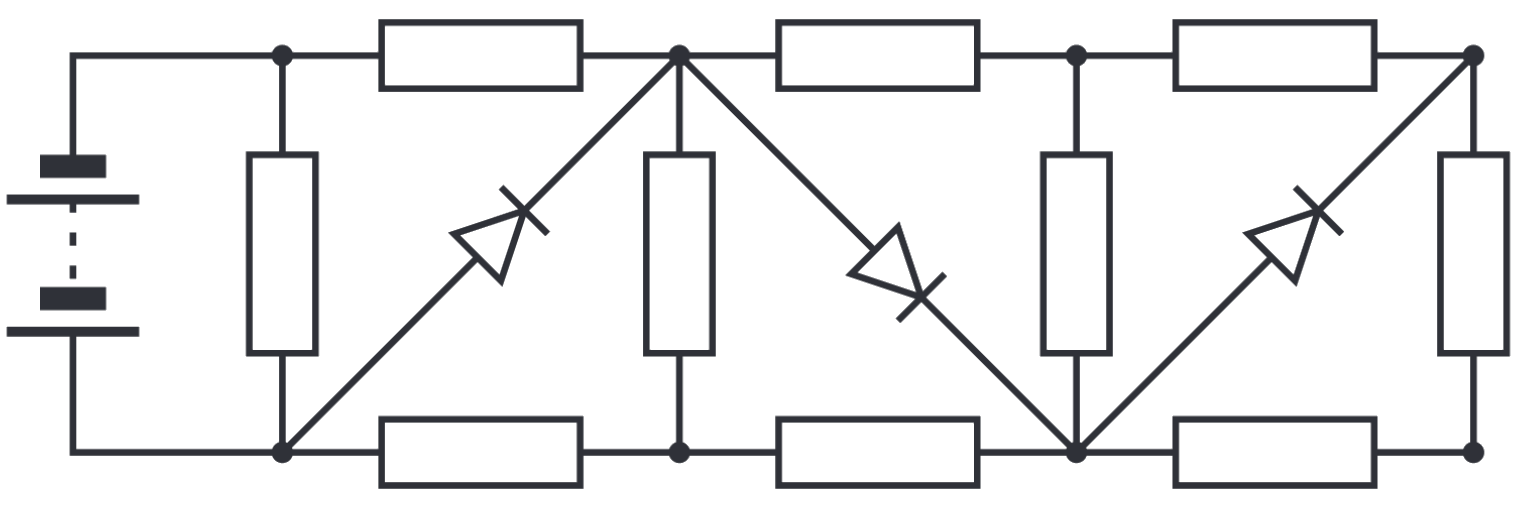
\includegraphics[width=0.8\textwidth]{S1 Figures/S1-34.png}
\end{center}
\end{solution}

\hypertarget{P35}{}
\begin{solution}{normal} % 35
Find the power dissipation on each of the diodes in the figure below. These diodes open at the forward voltage $V_0=1.0\;\text{V}$. It can be assumed that the diode voltage remains equal to $V_0$ for any forward current, and that for voltages less than $V_0$, there is no current through the diode, as shown in the figure below. The values of the resistances and of the electromotive force are given in the figure. (Kalda Circuits P29)
\begin{center}
    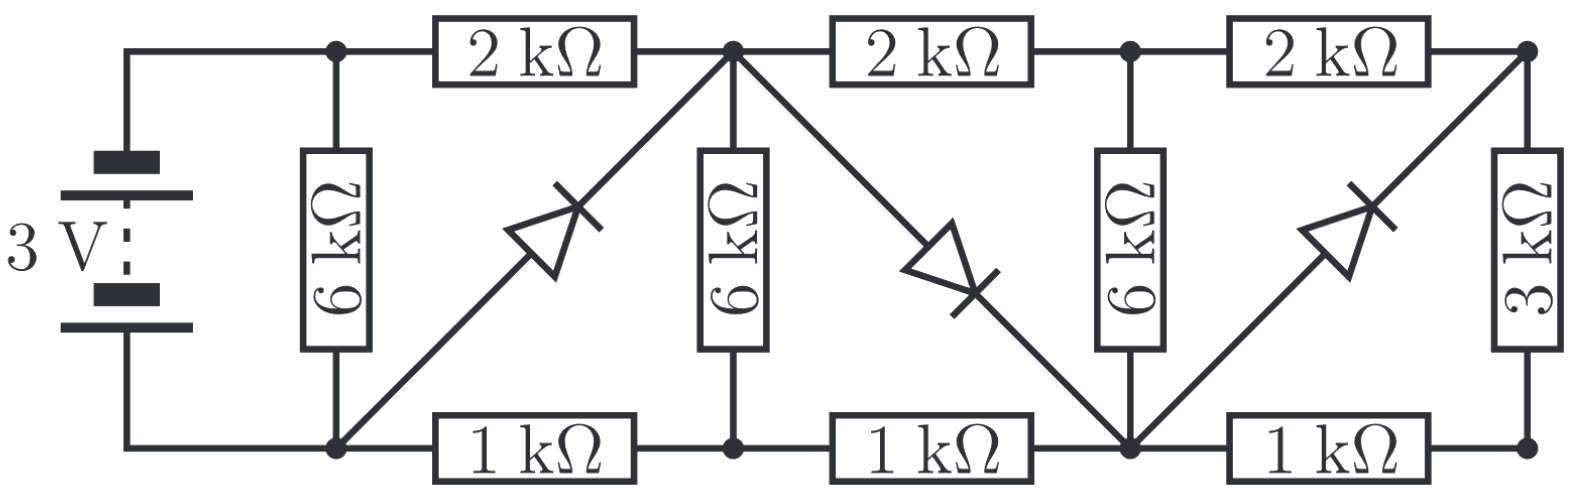
\includegraphics[width=0.8\textwidth]{S1 Figures/S1-35-1.png}
\end{center}
\begin{center}
    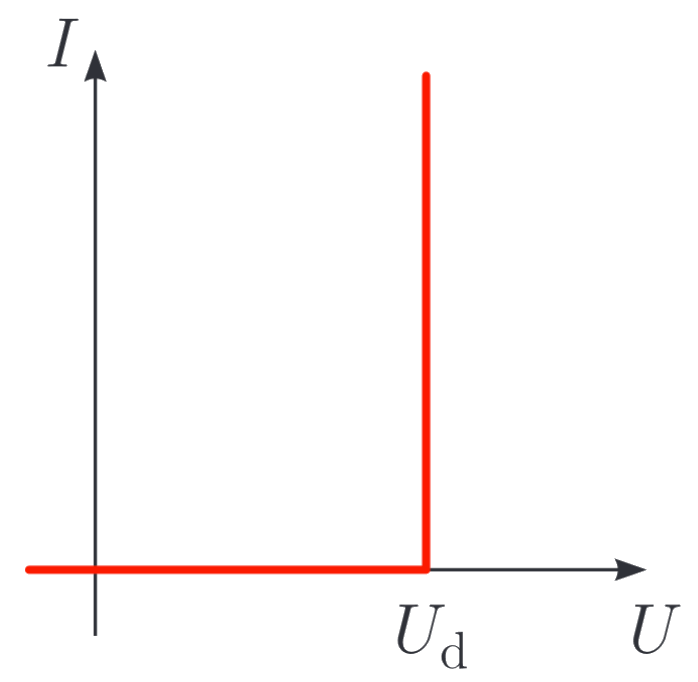
\includegraphics[width=0.4\textwidth]{S1 Figures/S1-35-2.png}
\end{center}
\end{solution}

\hypertarget{P36}{}
\begin{solution}{normal} % 36
Find the current in the circuit given below; the $I(V)$ dependence of the diode is shown in graph. (Kalda Circuits P24)
\begin{center}
    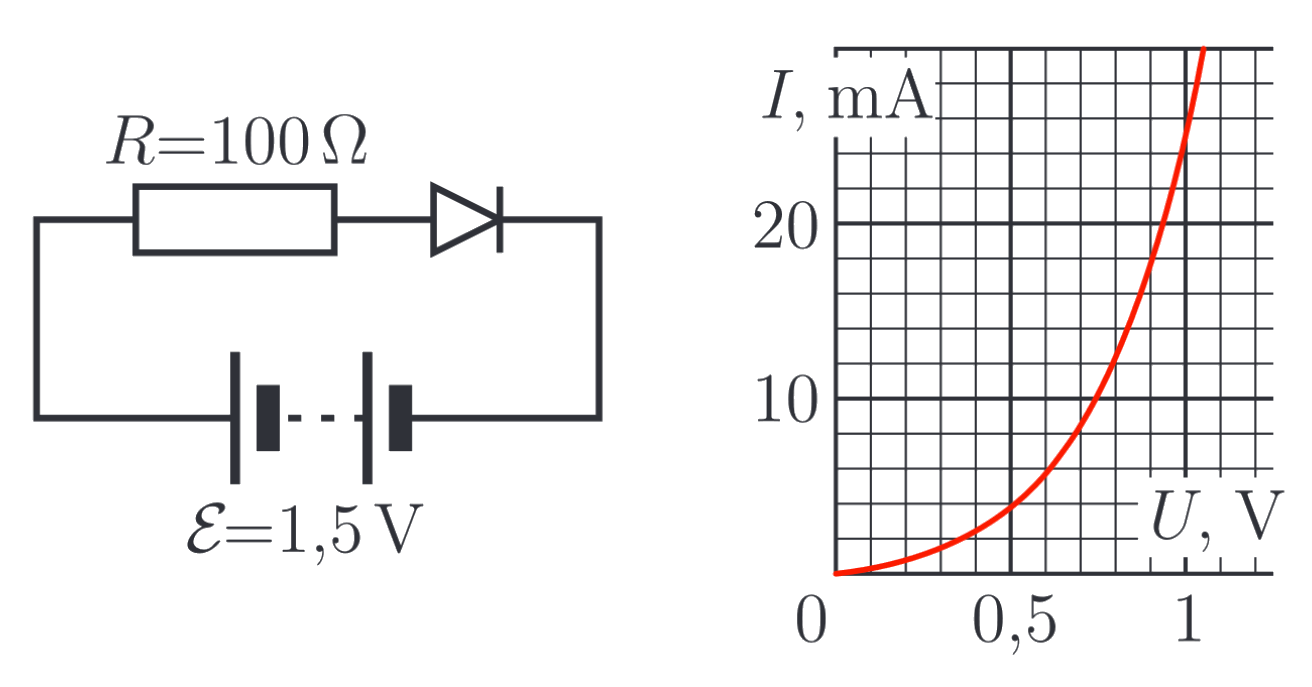
\includegraphics[width=0.75\textwidth]{S1 Figures/S1-36.png}
\end{center}
\end{solution}

\hypertarget{P37}{}
\begin{solution}{normal} % 37
Determine the current flowing through diode $D_2$ in the circuit below. The diodes are identical and have $I(V)$ dependence identical to the diode in Problem 36.
\begin{center}
    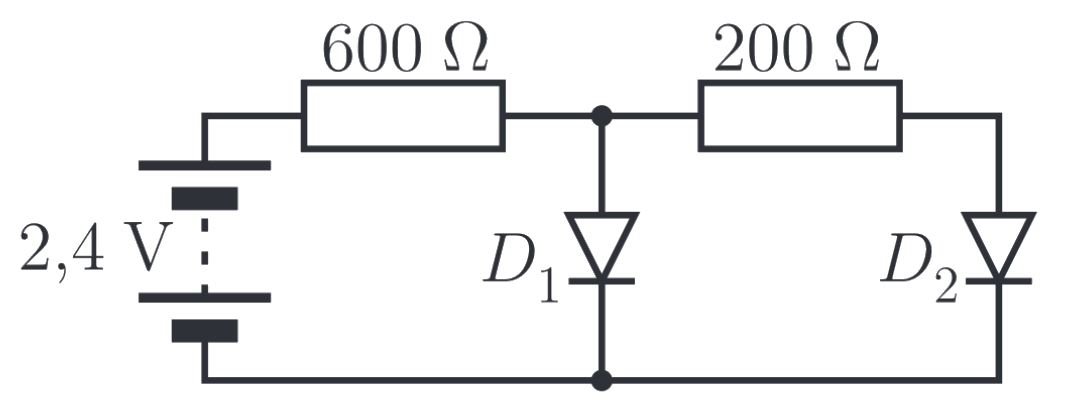
\includegraphics[width=0.6\textwidth]{S1 Figures/S1-37.png}
\end{center}
\end{solution}

\hypertarget{P38}{}
\begin{solution}{normal} % 38
The figure below shows the $I(V)$ dependence of the lamp, which is connected to the circuit as shown in the diagram below. How much power is dissipated by the lamp?
\begin{center}
    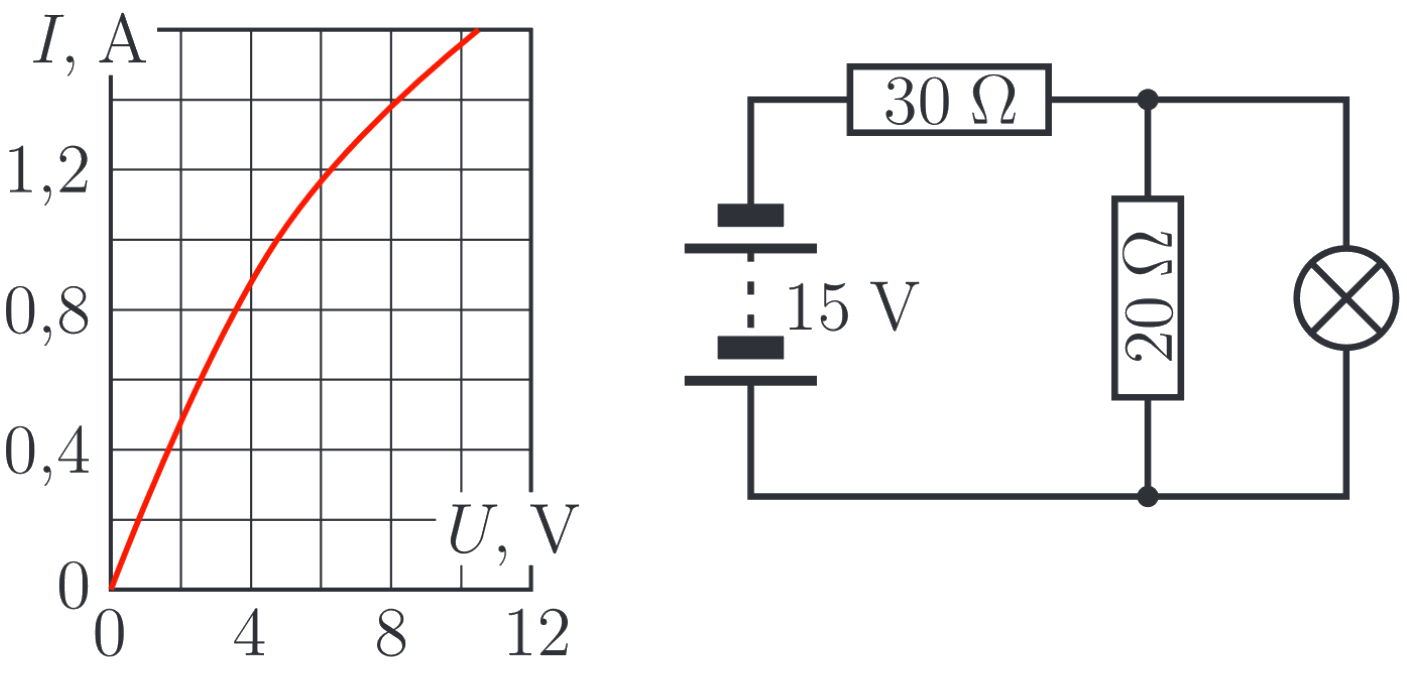
\includegraphics[width=0.75\textwidth]{S1 Figures/S1-38.png}
\end{center}
\end{solution}

\hypertarget{P39}{}
\begin{solution}{normal} % 39 ? unsure about translation
The $I-V$ curve of a thyristor is shown in the graph below. The thyristor is connected in series with a resistor of resistance $R$. What minimum voltage $U_0$ must be applied to the circuit for the thyristor to open (i.e. the current in the circuit increases exponentially)? Sketch the change in current in the circuit as the voltage applied increases linearly from $0$ to $U_0$ and back to $0$.
\begin{center}
    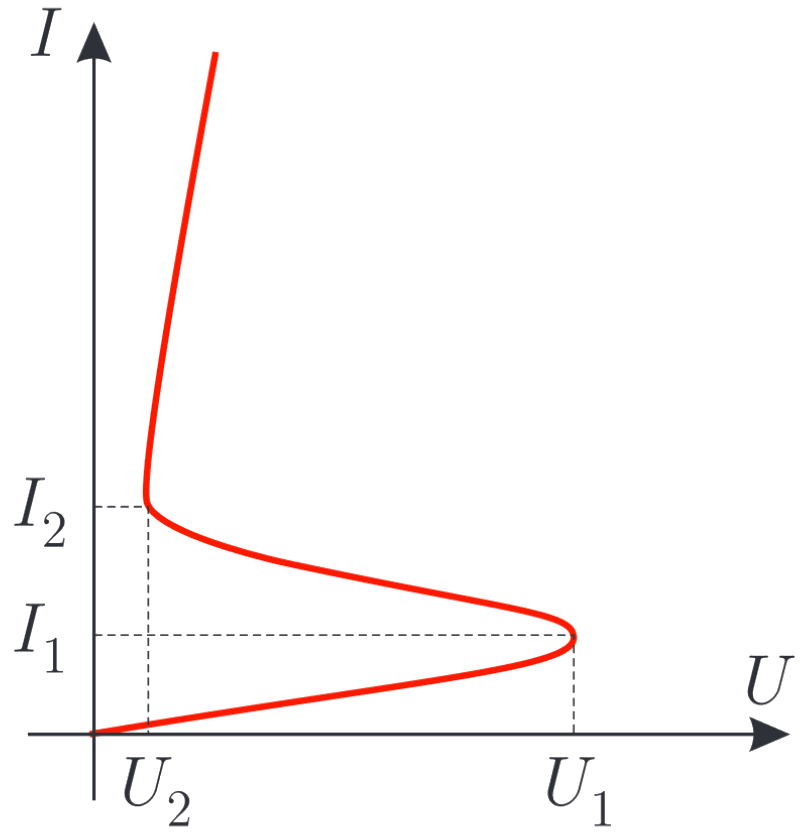
\includegraphics[width=0.4\textwidth]{S1 Figures/S1-39.png}
\end{center}
\end{solution}

\hypertarget{P40}{}
\begin{solution}{normal} % 40
In the figure below, the circuit of a simple tunnel-diode-based amplifier is given. Find the amplification factor for small-amplitude input signals using the following values. (Similar to Kalda Circuits P25)
\begin{center}
    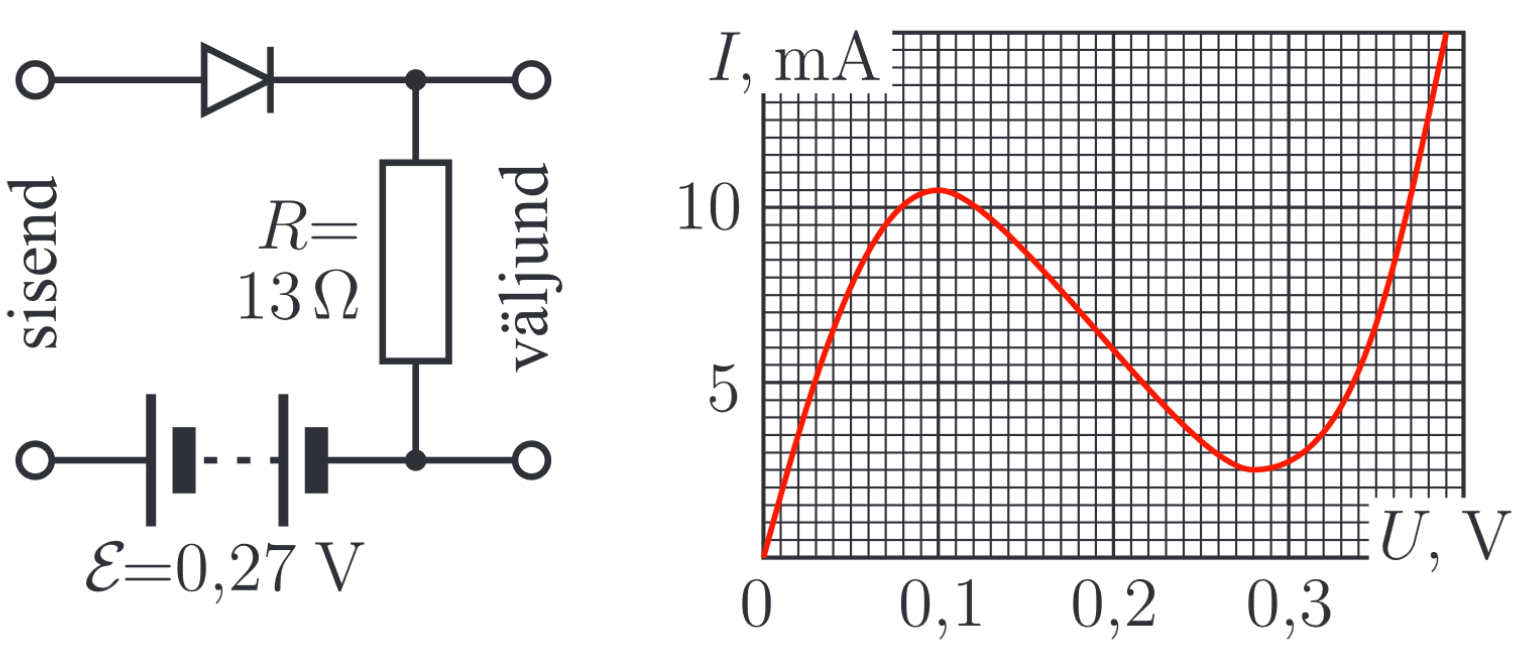
\includegraphics[width=0.7\textwidth]{S1 Figures/S1-40.png}
\end{center}
\end{solution}

\hypertarget{P41}{}
\begin{solution}{normal} % 41
To determine the current in a circuit, two ammeters with different measuring ranges are connected, one at a time. The ammeter with a measuring range of $10\;\text{mA}$ has a current reading of $2.95\;\text{mA}$ and the ammeter with a measuring range of $3\;\text{mA}$ has a current reading of $2.90\;\text{mA}$. What is the current in the circuit without an ammeter present? Assume that we are using a magnetoelectric ammeter with internal resistance inversely proportional to the measuring range. \textit{Note:} As the difference between the ammeter readings is relatively small, a linear approximation may be used and the change in current due to the additional resistance in the circuit (not due to the ammeter) can be considered to be proportional to the magnitude of the resistance.
\end{solution}

\hypertarget{P42}{}
\begin{solution}{normal} % 42
Show that if the resistance of an incandescent lamp is proportional to its (absolute) temperature, the current-voltage characteristic of the lamp is $I\propto U^{3/5}$.
\end{solution}

\hypertarget{P43}{}
\begin{solution}{normal} % 43
The label on a filament lamp  reads: $26\;\text{V},\;0.12\;\text{A}$. At room temperature, the resistance of the filament was measured to be $R_0=24\;\Omega$. Determine the length, diameter, and operating temperature of the filament. The filament is made of tungsten and has resistivity $\rho_0=5.3\times10^{-8}\;\Omega\;\text{m}$.
\end{solution}

\hypertarget{P44}{}
\begin{solution}{normal} % 44
The filament in a halogen light bulb is $5\;\text{cm}$ long. The filament is made of tungsten wire with density $19300\;\text{kg}/\text{m}^3$ and specific heat capacity $134\;\text{J}/(\text{kg}\cdot\text{K})$, which can be considered to be constant over the given temperature range. The resistivity of tungsten as a function of temperature is shown in the graph below. An excessive DC voltage of $120\;\text{V}$ is applied to the bulb. How long does it take to reach its melting point of $3410\degree\text{C}$?
\begin{center}
    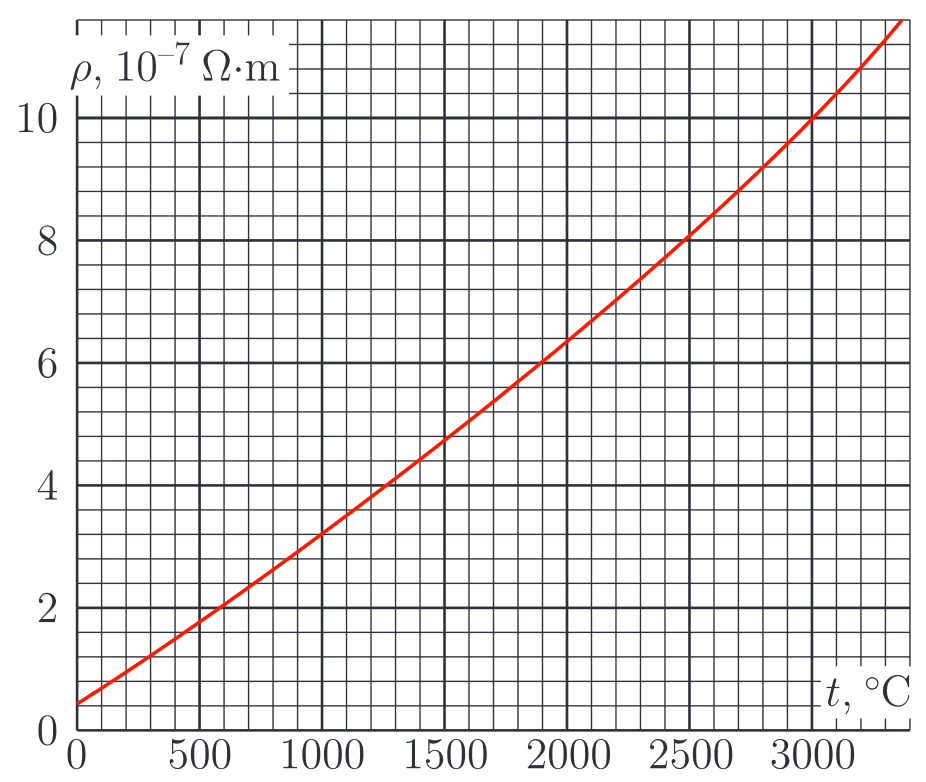
\includegraphics[width=0.7\textwidth]{S1 Figures/S1-44.png}
\end{center}
\end{solution}